%!TEX root = ../Proeycto.tex
\chapter{Marco de Referencia}

 Desde finales del siglo pasado, los avances tecnológicos en la miniaturización de la electrónica y los componentes mecánicos han allanado el camino para la creación y desarrollo de objetos voladores de pequeñas dimensiones, tales como aviones y helicópteros, los cuales están adquiriendo cada vez más habilidades para realizar vuelos de forma autónoma. Estos dispositivos son popularmente conocidos como drones, un término derivado del inglés \say{abejorros}, y se consideran máquinas voladoras autónomas o semi-autónomas capaces de llevar a cabo misiones de vuelo. En el ámbito internacional, se les conoce como UAVs del ingles \say{Unmanned Aerial Vehicles}, y representan una tecnología compleja cuyo control presenta desafíos, dado que sus características aerodinámicas son similares a las de las aeronaves convencionales \cite{eisenbeiss2004mini}.

El estudio de estos dispositivos despierta un gran interés debido a su versatilidad y capacidad de maniobra, lo que les permite llevar a cabo una amplia gama de tareas en diversas aplicaciones, tales como el uso civil, militar y aeroespacial \cite{nawaz2019applications, shakhatreh2019unmanned, xiaoning2020analysis}. En la figura \ref{fig1_aplicacion_UAV}, se presenta una clasificación detallada de las aplicaciones más importantes de los UAVs.

\begin{figure}[H]
    \centering
    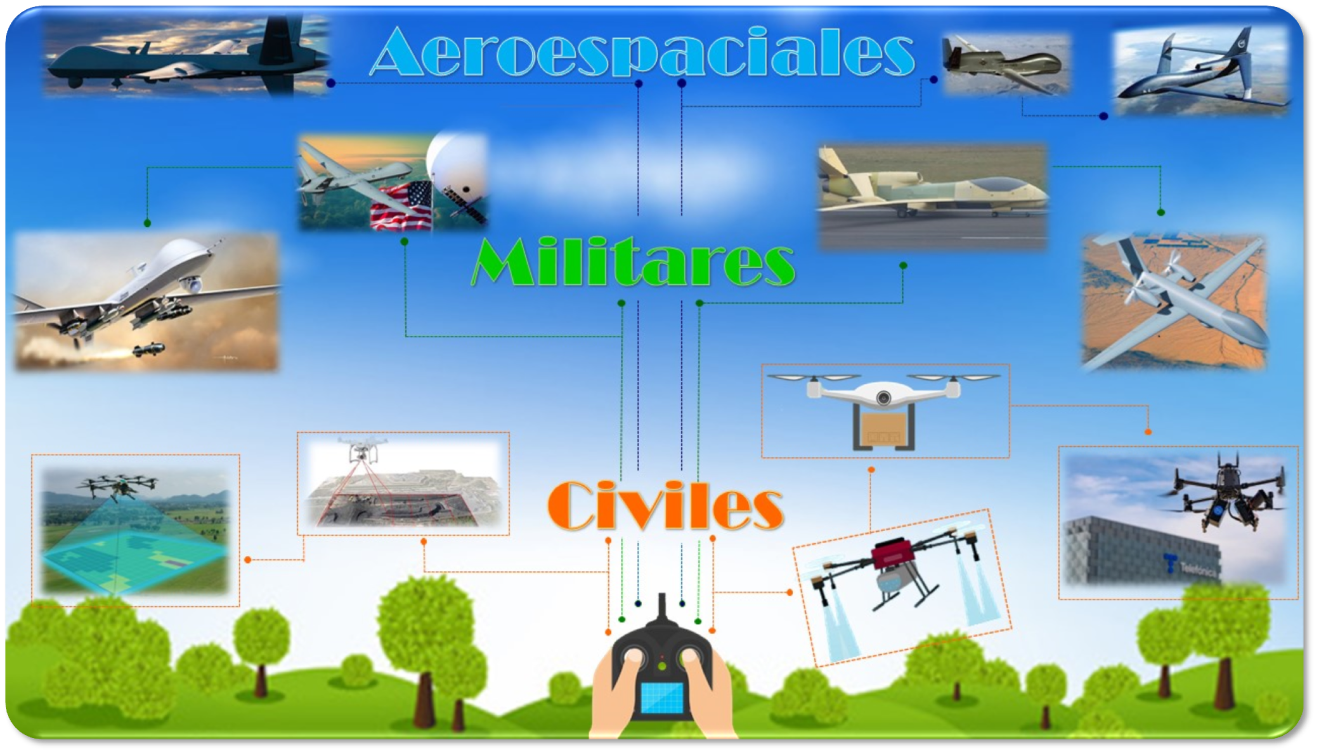
\includegraphics[width=16cm, height=7.5cm]{imagenes/Aplicaciones_UAV.png}
    \caption{Áreas de aplicación UAVS.}
    \label{fig1_aplicacion_UAV}
\end{figure}

\section{Antecedentes.}

Los drones han atraído la atención de la comunidad investigadora que trabaja tanto en el campo militar como en el civil, con una gran cantidad de usos que han sido propuestos por los grupos de investigación, debido a sus características como capacidad y configuraciones, donde el helicóptero de cuatro rotores tiene el mayor número de citas en la literatura de control y ha sido ampliamente investigado para pruebas tanto en interiores como en exteriores . 

\section{Objetivo General}

Desarrollar el sistema de citas trámites y expedientes como una plataforma web, segura y adaptable, que optimice la gestión de trámites gubernamentales mediante la automatización de citas, el control del acceso y la trazabilidad transaccional, garantizando la protección de los datos del ciudadano y la eficiencia operativa de los servidores públicos, facilitando el ordenamiento y la eficiencia del acceso de la ciudadanía a la realización y gestión de trámites de servicio públicos o privados.

\section{Objetivos Específicos}

\begin{itemize}
    \item Establecer un esquema de base de datos y migraciones optimizadas en Laravel para las entidades críticas del sistema (usuarios, roles, solicitud, asignación de revisor y bitácora) garantizando la integridad referencial, el almacenamiento estructurado de expediente y la gestión eficiente de relaciones de muchos a muchos para el control multi-rol.
    \item Desarrollar middlewares especializados en cifrado estricto en PHP 8.4 que garantice una autorización que restrinja la visualización y modificación de expedientes exclusivamente a sus propietarios legítimos o al personal técnico antes asignado y brinde acceso a las funciones administrativas.
    \item Diseñar la lógica de negocio y el flujo que permita a la ciudadanía realizar sus solicitudes de forma digital y autónoma mientras los revisores, supervisores y administradores operan bajo esquemas de asignación de cargas de trabajo.
\end{itemize}

\section{Alcance}

\begin{itemize}
    \item \textbf{Módulo de Autenticación y Usuarios:} Gestión de registro, inicio de sesión e identificación de perfiles institucionales (Ciudadano, Revisor, Supervisor, Administrador).
    \item \textbf{Módulo de Gestión de Expedientes y Citas:} Programación de citas y procesamiento del ciclo de vida de los trámites (creación, seguimiento, revisión y dictamen).
    \item \textbf{Seguridad y Control de Acceso:} Restricción de permisos por roles (\texttt{CheckRole}) y validación de acceso a expedientes por propiedad o asignación (\texttt{VerificarAccesoSolicitud}).
    \item \textbf{Módulo de Auditoría y Trazabilidad:} Registro automático en bitácora con marcas de tiempo, usuarios, ID y cargas útiles de operaciones de cambio (\texttt{RegistrarBitacora}).
\end{itemize}

\section{Limitaciones}

\begin{itemize}
    \item \textbf{Procesamiento de Pagos:} El sistema no contempla pasarelas de pago electrónico integradas; la validación de derechos y comprobantes se realiza de forma externa o presencial.
    \item \textbf{Infraestructura Tecnológica:} La disponibilidad operativa depende directamente de los servidores institucionales asignados y de la estabilidad de la red interna de la dependencia gubernamental.
    \item \textbf{Firma Electrónica:} No incluye certificación criptográfica avanzada ni integración con servicios federales de firma electrónica avanzada (FEA).
    \item \textbf{Canales de Acceso:} El acceso está estrictamente limitado a navegadores web estándar en plataformas de escritorio y dispositivos móviles, excluyendo el desarrollo de aplicaciones nativas.
    \item \textbf{Notificaciones por SMS o WhatsApp:} El envío de alertas y avisos de estatus sobre las citas y trámites se limita exclusivamente al correo electrónico institucional, omitiendo servicios de mensajería instantánea por red celular.
    \item \textbf{Almacenamiento de Archivos Adjuntos:} El tamaño de los archivos adjuntos en los expedientes (identificaciones, comprobantes, documentos de soporte) está restringido por las cuotas de almacenamiento configuradas en el servidor web.
    \item \textbf{Respaldo Externo:} El sistema manejará el resguardo de información únicamente mediante la bitácora.
\end{itemize}

\section{Problemática}

La problemática se centra en que la gestión presencial o mediante sistemas obsoletos provoca aglomeraciones en ventanillas, tiempos prolongados de atención, una deficiente distribución de las cargas de trabajo y la acumulación de documentación en papel a falta de un expediente digital centralizado, con lo cual incrementan los costos de archivo, consumo de insumos y riesgo de deterioro o pérdida de información física; asimismo, la ausencia de mecanismos de auditoría automatizados impide conocer con exactitud qué usuario o servidor público realizó modificaciones sobre un expediente, dificultando la rendición de cuentas y la transparencia institucional.

\section{Justificación}

El desarrollo del sistema se justifica como una solución integral que elimina la saturación en ventanillas, los tiempos de espera y el uso excesivo de papel mediante un expediente digital centralizado. Asimismo, incorpora un sistema de auditoría automatizado que garantiza la transparencia y la rendición de cuentas al registrar con exactitud cada modificación realizada por los usuarios.

